% Options for packages loaded elsewhere
\PassOptionsToPackage{unicode}{hyperref}
\PassOptionsToPackage{hyphens}{url}
\PassOptionsToPackage{dvipsnames,svgnames,x11names}{xcolor}
%
\documentclass[
  a4paper,
  DIV=11,
  numbers=noendperiod,
  oneside]{scrartcl}

\usepackage{amsmath,amssymb}
\usepackage{setspace}
\usepackage{iftex}
\ifPDFTeX
  \usepackage[T1]{fontenc}
  \usepackage[utf8]{inputenc}
  \usepackage{textcomp} % provide euro and other symbols
\else % if luatex or xetex
  \usepackage{unicode-math}
  \defaultfontfeatures{Scale=MatchLowercase}
  \defaultfontfeatures[\rmfamily]{Ligatures=TeX,Scale=1}
\fi
\usepackage{lmodern}
\ifPDFTeX\else  
    % xetex/luatex font selection
\fi
% Use upquote if available, for straight quotes in verbatim environments
\IfFileExists{upquote.sty}{\usepackage{upquote}}{}
\IfFileExists{microtype.sty}{% use microtype if available
  \usepackage[]{microtype}
  \UseMicrotypeSet[protrusion]{basicmath} % disable protrusion for tt fonts
}{}
\makeatletter
\@ifundefined{KOMAClassName}{% if non-KOMA class
  \IfFileExists{parskip.sty}{%
    \usepackage{parskip}
  }{% else
    \setlength{\parindent}{0pt}
    \setlength{\parskip}{6pt plus 2pt minus 1pt}}
}{% if KOMA class
  \KOMAoptions{parskip=half}}
\makeatother
\usepackage{xcolor}
\usepackage[top=2cm,bottom=4cm,left=2cm,right=2cm,heightrounded]{geometry}
\setlength{\emergencystretch}{3em} % prevent overfull lines
\setcounter{secnumdepth}{-\maxdimen} % remove section numbering
% Make \paragraph and \subparagraph free-standing
\makeatletter
\ifx\paragraph\undefined\else
  \let\oldparagraph\paragraph
  \renewcommand{\paragraph}{
    \@ifstar
      \xxxParagraphStar
      \xxxParagraphNoStar
  }
  \newcommand{\xxxParagraphStar}[1]{\oldparagraph*{#1}\mbox{}}
  \newcommand{\xxxParagraphNoStar}[1]{\oldparagraph{#1}\mbox{}}
\fi
\ifx\subparagraph\undefined\else
  \let\oldsubparagraph\subparagraph
  \renewcommand{\subparagraph}{
    \@ifstar
      \xxxSubParagraphStar
      \xxxSubParagraphNoStar
  }
  \newcommand{\xxxSubParagraphStar}[1]{\oldsubparagraph*{#1}\mbox{}}
  \newcommand{\xxxSubParagraphNoStar}[1]{\oldsubparagraph{#1}\mbox{}}
\fi
\makeatother


\providecommand{\tightlist}{%
  \setlength{\itemsep}{0pt}\setlength{\parskip}{0pt}}\usepackage{longtable,booktabs,array}
\usepackage{calc} % for calculating minipage widths
% Correct order of tables after \paragraph or \subparagraph
\usepackage{etoolbox}
\makeatletter
\patchcmd\longtable{\par}{\if@noskipsec\mbox{}\fi\par}{}{}
\makeatother
% Allow footnotes in longtable head/foot
\IfFileExists{footnotehyper.sty}{\usepackage{footnotehyper}}{\usepackage{footnote}}
\makesavenoteenv{longtable}
\usepackage{graphicx}
\makeatletter
\def\maxwidth{\ifdim\Gin@nat@width>\linewidth\linewidth\else\Gin@nat@width\fi}
\def\maxheight{\ifdim\Gin@nat@height>\textheight\textheight\else\Gin@nat@height\fi}
\makeatother
% Scale images if necessary, so that they will not overflow the page
% margins by default, and it is still possible to overwrite the defaults
% using explicit options in \includegraphics[width, height, ...]{}
\setkeys{Gin}{width=\maxwidth,height=\maxheight,keepaspectratio}
% Set default figure placement to htbp
\makeatletter
\def\fps@figure{htbp}
\makeatother
% definitions for citeproc citations
\NewDocumentCommand\citeproctext{}{}
\NewDocumentCommand\citeproc{mm}{%
  \begingroup\def\citeproctext{#2}\cite{#1}\endgroup}
\makeatletter
 % allow citations to break across lines
 \let\@cite@ofmt\@firstofone
 % avoid brackets around text for \cite:
 \def\@biblabel#1{}
 \def\@cite#1#2{{#1\if@tempswa , #2\fi}}
\makeatother
\newlength{\cslhangindent}
\setlength{\cslhangindent}{1.5em}
\newlength{\csllabelwidth}
\setlength{\csllabelwidth}{3em}
\newenvironment{CSLReferences}[2] % #1 hanging-indent, #2 entry-spacing
 {\begin{list}{}{%
  \setlength{\itemindent}{0pt}
  \setlength{\leftmargin}{0pt}
  \setlength{\parsep}{0pt}
  % turn on hanging indent if param 1 is 1
  \ifodd #1
   \setlength{\leftmargin}{\cslhangindent}
   \setlength{\itemindent}{-1\cslhangindent}
  \fi
  % set entry spacing
  \setlength{\itemsep}{#2\baselineskip}}}
 {\end{list}}
\usepackage{calc}
\newcommand{\CSLBlock}[1]{\hfill\break\parbox[t]{\linewidth}{\strut\ignorespaces#1\strut}}
\newcommand{\CSLLeftMargin}[1]{\parbox[t]{\csllabelwidth}{\strut#1\strut}}
\newcommand{\CSLRightInline}[1]{\parbox[t]{\linewidth - \csllabelwidth}{\strut#1\strut}}
\newcommand{\CSLIndent}[1]{\hspace{\cslhangindent}#1}


\usepackage{float}
\floatplacement{table}{H}

\usepackage{caption}

\captionsetup{justification=raggedright,singlelinecheck=false}

\usepackage{lipsum}

\usepackage{icomma}
\usepackage{siunitx}
\sisetup{
  add-decimal-zero = false , % default setting, not needed
  output-decimal-marker = {,} ,
  group-separator = \, % default setting, not needed
}

% gt packages

\usepackage{booktabs}
\usepackage{caption}
\usepackage{longtable}
\usepackage{colortbl}
\usepackage{array}
\usepackage{anyfontsize}
\usepackage{multirow}
\usepackage{lastpage}
\usepackage{fancyhdr}

\fancypagestyle{fancy}{
 \fancyhf{} % clear all header and footer fields
 \fancyfoot[C]{Side \thepage\ af \pageref*{LastPage}}
 \renewcommand{\headrulewidth}{0pt}
 \renewcommand{\footrulewidth}{0pt}
}
\fancypagestyle{plain}{
 \fancyhf{}
 \fancyfoot[C]{Side \thepage\ af \pageref*{LastPage}}
 \renewcommand{\headrulewidth}{0pt}
 \renewcommand{\footrulewidth}{0pt}
}
\pagestyle{fancy}
\KOMAoption{captions}{tableheading}
\makeatletter
\@ifpackageloaded{caption}{}{\usepackage{caption}}
\AtBeginDocument{%
\ifdefined\contentsname
  \renewcommand*\contentsname{Indholdsfortegnelse}
\else
  \newcommand\contentsname{Indholdsfortegnelse}
\fi
\ifdefined\listfigurename
  \renewcommand*\listfigurename{Figuroversigt}
\else
  \newcommand\listfigurename{Figuroversigt}
\fi
\ifdefined\listtablename
  \renewcommand*\listtablename{Tabeloversigt}
\else
  \newcommand\listtablename{Tabeloversigt}
\fi
\ifdefined\figurename
  \renewcommand*\figurename{Figur}
\else
  \newcommand\figurename{Figur}
\fi
\ifdefined\tablename
  \renewcommand*\tablename{Tabel}
\else
  \newcommand\tablename{Tabel}
\fi
}
\@ifpackageloaded{float}{}{\usepackage{float}}
\floatstyle{ruled}
\@ifundefined{c@chapter}{\newfloat{codelisting}{h}{lop}}{\newfloat{codelisting}{h}{lop}[chapter]}
\floatname{codelisting}{Liste}
\newcommand*\listoflistings{\listof{codelisting}{Listeoversigt}}
\makeatother
\makeatletter
\makeatother
\makeatletter
\@ifpackageloaded{caption}{}{\usepackage{caption}}
\@ifpackageloaded{subcaption}{}{\usepackage{subcaption}}
\makeatother
\makeatletter
\@ifpackageloaded{sidenotes}{}{\usepackage{sidenotes}}
\@ifpackageloaded{marginnote}{}{\usepackage{marginnote}}
\makeatother

\ifLuaTeX
\usepackage[bidi=basic]{babel}
\else
\usepackage[bidi=default]{babel}
\fi
\babelprovide[main,import]{danish}
% get rid of language-specific shorthands (see #6817):
\let\LanguageShortHands\languageshorthands
\def\languageshorthands#1{}
\ifLuaTeX
  \usepackage{selnolig}  % disable illegal ligatures
\fi
\usepackage{bookmark}

\IfFileExists{xurl.sty}{\usepackage{xurl}}{} % add URL line breaks if available
\urlstyle{same} % disable monospaced font for URLs
\hypersetup{
  pdftitle={Sådan installerer du et nyt output-format i Zotero},
  pdfauthor={Aleksander Bang-Larsen},
  pdflang={da},
  colorlinks=true,
  linkcolor={blue},
  filecolor={Maroon},
  citecolor={Blue},
  urlcolor={Blue},
  pdfcreator={LaTeX via pandoc}}


\title{Sådan installerer du et nyt output-format i Zotero}
\author{Aleksander Bang-Larsen}
\date{2024-05-17}

\begin{document}
\maketitle

\renewcommand*\contentsname{Indholdsfortegnelse}
{
\hypersetup{linkcolor=}
\setcounter{tocdepth}{3}
\tableofcontents
}

\setstretch{1.5}
\subsection{Baggrund}\label{baggrund}

Denne guide er beregnet til dig, der er interesseret i, hvordan man
installerer et \emph{custom} output i Zotero. Måske er du blevet henvist
hertil er blevet vist hertil og har fået tilsendt mit speciallavede
politica-output til Zotero. Her vil du finde vejledning til, hvordan du
importerer og bruger den med dine henvisninger.

Denne guide tager udgangspunkt i, at du allerede har Zotero 6
installeret. Du kan downloade Zotero på programmets
\href{https://www.zotero.org/download/}{hjemmeside}.

\subsection{Ting du skal igennem}\label{ting-du-skal-igennem}

\begin{itemize}
\tightlist
\item
  Downloade csl filer og placere et smart sted (f.eks. sammen med
  zotero)
\item
  Installere output-formatet
\item
  Vælge det som default output
\item
  Bruge output i word
\end{itemize}

\subsection{Download og placering af
csl-filer}\label{download-og-placering-af-csl-filer}

Du skal sørge for, at filerne ligger et sted, hvor du kan finde dem. Jeg
har mine til at ligge i OneDrive sammen med mine andre dokumenter.

\marginnote{\begin{footnotesize}

\begin{figure}[tbh]

{\centering 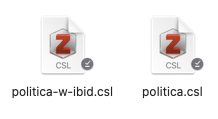
\includegraphics{images/filer-light.png}

}

\caption{De to filer der skal gemmes}

\end{figure}%

\end{footnotesize}}

Hvis du ikke allerede har fået tilsendt \texttt{csl} filerne, kan du
hente dem ude til højre.

\subsubsection{\texorpdfstring{Hvad er forskellen på \texttt{politica}
og
\texttt{politica-w-ibid}?}{Hvad er forskellen på politica og politica-w-ibid?}}\label{hvad-er-forskellen-puxe5-politica-og-politica-w-ibid}

\texttt{politica.csl} er den stil du skal bruge, hvis du ikke ønsker at
Zotero laver \emph{ibid} automatisk eller du ønsker manuelt at skrive
ibid. \texttt{politica-w-ibid.csl} er den stil du skal bruge, hvis du
ønsker at Zotero automatisk indsætter \emph{ibid} når du bruger den
samme reference to gange i træk; og tæt på hinanden.

\subsection{Installation af output}\label{installation-af-output}

For at installere output-stilen skal du blot dobbeltklikke på
\texttt{csl} filen på dit drev. Så får du denne besked op:

\begin{figure}[tbh]

{\centering 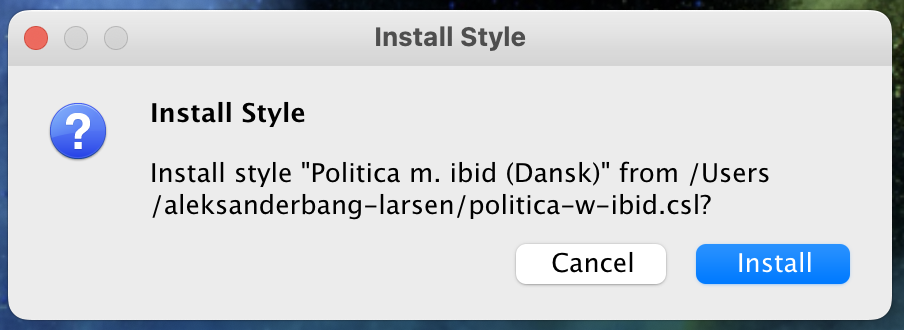
\includegraphics{images/output-install.png}

}

\caption{Sådan skal det se ud, når du prøver at installere output}

\end{figure}%

Her skal du trykke \texttt{Install} og så vil stilen automatisk
installeres. Det skal du gentage for alle de output-stiler du vil
installere.

\marginnote{\begin{footnotesize}

Hint: Du kan tjekke de output-stiler der er installeret ved at gå i
\texttt{Settings} og under \texttt{Cite} er alle tilgængelige
output-stile listet.

\end{footnotesize}}

\subsection{Brug af output}\label{brug-af-output}

For at du kan bruge din output-stil skal du have nogle referencer klar i
Zotero. Jeg har valgt nedenstående:

\begin{itemize}
\tightlist
\item
  Togeby (2003)
\item
  Mouritsen (2009)
\item
  Midtgaard (2011)
\item
  Petersen et al. (2007)
\item
  Bush (2008)
\end{itemize}

I bunden af denne side kan du se en litteraturliste med disse
henvisninger i fuld format - Og der kan du også se om output-stilen
stemmer overens med Politicas skrivevejledning.

\subsubsection{Word}\label{word}

\subsection{FAQ}\label{faq}

\subsubsection{Jeg har fundet en fejl i outputtet - Hvad gør
jeg?}\label{jeg-har-fundet-en-fejl-i-outputtet---hvad-guxf8r-jeg}

\begin{itemize}
\tightlist
\item
  Hvis du har fundet en fejl i en af de styles jeg har produceret kan du
  sende mig en mail eller tage fat på mig \emph{IRL} eller på diverse
  sociale medier.
\item
  Hvis der er tale om en fejlimplementering i forhold til
  \href{https://politica.dk/bidrag-til-politica/skrivevejledning-for-politica/}{skrivevejledningen
  fra politica} retter jeg den med glæde.

  \begin{itemize}
  \tightlist
  \item
    Ellers kan vi tale om at producere en stil der passer til dine
    ønsker.
  \end{itemize}
\item
  Når du kontakter mig vedrørende en fejl er det en god ide at sende din
  csl-fil med; det gør det nemlig nememre at finde ud af, hvad fejlen er
  og hvor den findes.
\end{itemize}

\subsubsection{Hvorfor kan jeg ikke bare downloade output-stilen inde i
Zotero som man kan med
andre?}\label{hvorfor-kan-jeg-ikke-bare-downloade-output-stilen-inde-i-zotero-som-man-kan-med-andre}

\begin{itemize}
\tightlist
\item
  Jeg arbejder på at få denne output-stil integreret i den primære
  downloadside, men det kræver at CSL-projektet vil acceptere den. Du
  kan læse mere om, hvad det kræver
  \href{https://github.com/citation-style-language/styles/blob/master/README.md\#criteria-for-inclusion}{her}.
  Du kan også følge med i processen
  \href{https://github.com/citation-style-language/styles/pull/6797}{her}.
\end{itemize}

\phantomsection\label{refs}
\begin{CSLReferences}{1}{1}
\bibitem[\citeproctext]{ref-bush2008}
Bush, George W. (2008). President {Bush Addresses United Nations General
Assembly}. {Office} of the {Press Secretary}. {September} 23. The United
Nations, New York, januar, 2008.

\bibitem[\citeproctext]{ref-midtgaard2011}
Midtgaard, Søren Flinch (2011). {Retf{æ}rdighedens omst{æ}ndigheder}.
\emph{Politica} 43 (3): 334--351.

\bibitem[\citeproctext]{ref-mouritsen2009}
Mouritsen, Per (2009). Den Nationale Borger. pp. 80--86 i Jens
Blom-Hansen og Jørgen Elklit (red). \emph{Perspektiver P{å} Politik},
Aarhus: Academica.

\bibitem[\citeproctext]{ref-petersen2007}
Petersen, Michael Bang, Rune Slothuus, Rune Stubager og Lise Togeby
(2007). Hvem Fortjener Velf{æ}rd? {Danskernes} Syn P{å} Kontanthj{æ}lp
Til Unge, {Æ}ldre Og Indvandrere. \emph{Politica} 39 (1): 31--48.

\bibitem[\citeproctext]{ref-togeby2003}
Togeby, Lise (2003). \emph{{Fra fremmedarbejdere til etniske
minoriteter}}. {Å}rhus: Aarhus Universitetsforlag.

\end{CSLReferences}




\end{document}
